% !TEX root = ../main.tex
\section{Textual Labels}
\label{sec:linguistic-labels}

Once the time locations where inputs and outputs are sampled is determined, one must choose suitable input labels for the prediction of the target outputs. 

In this section, I present each set of linguistic labels that are included in the proposed methodology and describe their role and usefulness for the task of \ac{F0} modeling.
Finally, I present how they are converted into their corresponding binary features and combined into input vectors for the \ac{DNN} model.

\subsection{Phones}

Even at the lowest level, i.e., at the level of the phonemes, \ac{F0} is affected. 
At this level, depending on the phoneme and the amount of voicing applied to its corresponding phonemic realization, pitch features might or might not be specified. 

This inconvenient fact is often circumvented by interpolating the missing \ac{F0} measurements and applying smoothing. 
Critics of this approach point out that this produces artifacts that might negatively affect the learning process and the results \citep{Wang2017RNN}.

In the proposed methodology, each intonational event represents a movement describing the amount of pitch change from the previously observed \ac{F0} value (for more details on the \ac{F0} encoding, see \autoref{sec:f0-encoding}).
If the frequency of the previous value is unspecified (because it has not been interpolated), then it is impossible to calculate the amount of relative change between it and the currently observed \ac{F0} value.
This means that in the proposed methodology, it is not possible to do away with interpolation.
As \ac{F0} must always be interpolated, it is not necessary to include information about phonemes to account for unvoiced parts of the contour.
For these reasons, information about phones is not included.


\subsection{Onset and Rhyme}

In addition to the issue relating to whether phonemes are voiced or not, we also need to take into account that the timing of certain prosodic events might be tied to the structure of the syllable, as different parts of the syllable carry different amounts of prosodic information.
Consider for instance the phrase ``steak?", where most of the prosodic information (i.e., the upward inflection) is carried by the vowel (i.e., the nucleus) and not the fricative (i.e., the onset).

This issue cannot simply be addressed by including positional information such as percentage values.
Percentage values are not very reliable for syllables, because the internal structure of the syllable can change dramatically depending on the identity and relative duration of the phones it contains.

In order to better account for these timing phenomena and to ensure better alignment between the syllabic structure and the \ac{F0} contour, I decided to include onset and rhyme labels.



\subsection{Syllable}

Because of the importance of syllabic units, I included labels for both lexical stress (i.e., primary, secondary, and no stress) as well as syllable boundaries (i.e., either present or absent).

\subsection{\ac{POS} tags}

The next linguistic label I decided to include is \ac{POS} tags.
These are necessary in order to capture prosodic events pertaining to the syntactic domain. 
Phonologically identical words (e.g., the word ``cut'' can function both as a noun or a verb) often have different syntactic functions depending their \ac{POS} tag and correspondingly different prosodic behaviors.

Intuitively, a verb like ``to wrap'' behaves more closely to other verbs than the word ``wrap'' used as a noun. 
Notice how in the following sentences we can switch the verbs coming after ``want to'' and maintain the same overall prosodic profile (provided the new word has the same accent groups).

\begin{exe}
    \ex Tonight I want to \textbf{make} a few presents.
    \ex Tonight I want to \textbf{wrap} a few presents.
    \ex Tonight I want to \textbf{send} a few presents.
\end{exe}


\subsection{Lemmata}

The next set of labels I included in my implementation is word lemmata and word boundaries. 
This might seem like an unnecessary complication since word vectors will greatly increase the size of the model. 

The reason why word information is important is that words (especially used in context) can carry with them the semantics of a sentence as well the underlying attitude of a speaker who might decide to speak such an utterance.
For instance a speaker uttering ``I am so depressed today!'' is more likely to use a generally flatter and monotonous tone than someone who's uttering ``I feel so alive today!''.

Another reason it is desirable to include word vectors is that a lot of syntactic classes described by \ac{POS} tags are not fine-grained enough to capture important semantic and syntactic differences.
For instance, adverbial expressions such as ``additionally'', ``clearly'', ``not'', ``then'', ``yesterday'' are all labeled as part of the same group, even though they display very different syntactic behaviors, which can often lead to very different intonation patterns. 

In most language models, word vectors are not usually learned using vanilla softmax classification. 
This is due to the extremely large number of possible outputs (i.e., context words), which makes training very resource-intensive and time-consuming. 
A common workaround to this issue is to use noise classifiers \citep{Mikolov2013Distributed}. 
In our particular case, we will show that we have a fairly small number of output classes (for more details on the output of the proposed intonation model, see \autoref{sec:f0-encoding}), which means we are able to train word vectors using standard loss functions.

As adding words embeddings to the model is computationally expensive, it is important to select and process the word tokens carefully.
Morphological information is redundant, as it is by and large already encoded by the \ac{POS} tags.
Therefore it can be discarded by means of lemmatization.

Secondly, it is important to remove word lemmata that are only frequent as a mere consequence of the specific word distribution of the training corpus, e.g., character names, place names, etc.
These words are only specific to the training corpus.
It is therefore unlikely that they will come up again and that they will generalize well within new contexts.
To remove these words, we filter out the lemmata that are not found in frequency lists of English based on much larger corpora.\footnote{The frequency list used to filter out words is derived from the the British National Corpus (\url{http://www.natcorp.ox.ac.uk/using/index.xml?ID=freq}).}


\subsection{Punctuation}

The last feature I added to my implementation is punctuation. 
Punctuation, aside from helping distinguish between sentence types (interrogative, declarative, exclamatory, etc.) is a feature that is also useful for demarcating syntactic phrases and solving syntactic ambiguities. 
This in turn can help us decide which prosodic strategy to adopt. 

Since punctuation does not have a reliable acoustic representation (occasionally realized through pauses), punctuation annotations are added in correspondence to the words.
In particular, for every word, I added a label for punctuation before and after the word.
In the case of punctuation before the current word, the punctuation label is generated by concatenating all the text characters between the current word and the previous word.
Similarly, for the punctuation after the current word, the punctuation label is generated by concatenating all the text characters between the current word and the next word.
White space interspersing punctuation characters is removed.
The resulting punctuation labels are then augmented with a special punctuation label for no punctuation.


\subsection{Input vectors}
\label{input-vectors}

Linguistic labels cannot be used directly and fed to a neural network, as neural networks can only accept data in the form of input vectors.

In our case, most of our data is not sequences of numerical values, but rather categorical data such as words, stress information, \ac{POS} tags, etc.
In order to use this information, we first need to encode these values into one-hot vectors.
In one-hot vectors, all positions contain zeros, except for the position referring to the observed label, which contains a one.
This process converts the categorical data into binary features, that can be used by the neural network.
Based on the corpus used in the implementation, the binary features reported in \autoref{tab:ling-feat-f0} were obtained (for more details see \autoref{chap:appendix-a} and \autoref{chap:appendix-b}).


\begin{table}[h!]
  \centering
  \begin{tabular}{llc}
    \toprule
    \textbf{Level} & \textbf{Description} & \textbf{Size} \\
    \midrule
    Word     & lemmata                 & 1937 \\
             & \acs{POS} tags          &   66 \\
             & word boundaries         &    3 \\
             & punctuation before word &   55 \\
             & punctuation after word  &   55 \\
    \midrule
    Syllable & syllable boundaries     &    3 \\
             & syllable stress         &    5 \\
             & onset/rhyme             &    3 \\
    \bottomrule
  \end{tabular}
    \caption[Intonation model textual features.]{Linguistic features used as input for the \acs{F0}-\acs{DNN} model.}
  \label{tab:ling-feat-f0}
\end{table}


Binary features encoding various linguistic information can then be strung together into a single larger vector.
This is what is usually done in most neural network applications.

In the proposed approach, I followed a similar approach, with the difference that I decided to separate word vectors from the other linguistic inputs (see \autoref{fig:input-vector}).
This choice was primarily made for the sake of performance at inference time (for details, see \autoref{chap:intonation-modeling}).
Word vectors have an extremely high number of binary features and constitute the most expensive part of the model.



\begin{figure}[H]
\centering
\scalebox{0.9}{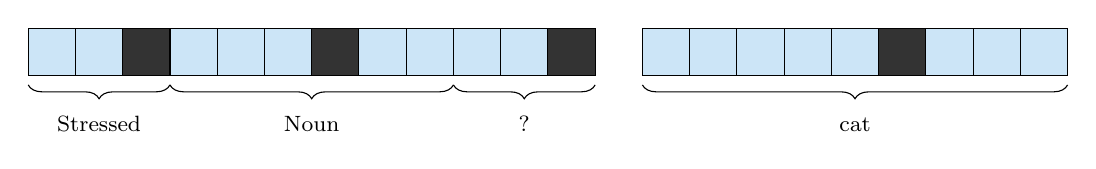
\begin{tikzpicture}[scale=1.2]

\filldraw[fill=cyan!80!blue!20!white, draw=black] 
(0,0) rectangle (0.5, 0.5);

\filldraw[fill=cyan!80!blue!20!white, draw=black] 
(0.5,0) rectangle (1, 0.5);

\filldraw[fill=black!80!white, draw=black] 
(1,0) rectangle (1.5, 0.5);

\filldraw[fill=cyan!80!blue!20!white, draw=black] 
(1.5,0) rectangle (2, 0.5);

\filldraw[fill=cyan!80!blue!20!white, draw=black] 
(2,0) rectangle (2.5, 0.5);

\filldraw[fill=cyan!80!blue!20!white, draw=black] 
(2.5,0) rectangle (3, 0.5);

\filldraw[fill=black!80!white, draw=black] 
(3,0) rectangle (3.5, 0.5);

\filldraw[fill=cyan!80!blue!20!white, draw=black] 
(3.5,0) rectangle (4, 0.5);

\filldraw[fill=cyan!80!blue!20!white, draw=black] 
(4,0) rectangle (4.5, 0.5);

\filldraw[fill=cyan!80!blue!20!white, draw=black] 
(4.5,0) rectangle (5, 0.5);

\filldraw[fill=cyan!80!blue!20!white, draw=black] 
(5,0) rectangle (5.5, 0.5);

\filldraw[fill=black!80!white, draw=black] 
(5.5,0) rectangle (6, 0.5);


\filldraw[fill=cyan!80!blue!20!white, draw=black] 
(6.5,0) rectangle (7, 0.5);

\filldraw[fill=cyan!80!blue!20!white, draw=black] 
(7,0) rectangle (7.5, 0.5);

\filldraw[fill=cyan!80!blue!20!white, draw=black] 
(7.5,0) rectangle (8, 0.5);

\filldraw[fill=cyan!80!blue!20!white, draw=black] 
(8,0) rectangle (8.5, 0.5);

\filldraw[fill=cyan!80!blue!20!white, draw=black] 
(8.5,0) rectangle (9, 0.5);

\filldraw[fill=black!80!white, draw=black] 
(9,0) rectangle (9.5, 0.5);

\filldraw[fill=cyan!80!blue!20!white, draw=black] 
(9.5,0) rectangle (10, 0.5);

\filldraw[fill=cyan!80!blue!20!white, draw=black] 
(10,0) rectangle (10.5, 0.5);

\filldraw[fill=cyan!80!blue!20!white, draw=black] 
(10.5,0) rectangle (11, 0.5);


\draw [decorate,decoration={brace,mirror,amplitude=5pt}]
    (0,-0.1) -- (1.5,-0.1) node [midway,yshift=-0.5cm] {\footnotesize{Stressed}};

\draw [decorate,decoration={brace,mirror,amplitude=5pt}]
    (1.5,-0.1) -- (4.5,-0.1) node [midway,yshift=-0.5cm] {\footnotesize{Noun}};

\draw [decorate,decoration={brace,mirror,amplitude=5pt}]
    (4.5,-0.1) -- (6.0,-0.1) node [midway,yshift=-0.5cm] {\footnotesize{?}};

\draw [decorate,decoration={brace,mirror,amplitude=5pt}]
    (6.5,-0.1) -- (11,-0.1) node [midway,yshift=-0.5cm] {\footnotesize{cat}};

\end{tikzpicture}}
\caption[Example of an input vector]{Example of an input vector.
Word and non-word features are encoded by two separate vectors.
This particular set of vectors could refer to a data point sampled at the end of a sentence such as ``Where is the cat?''.
}
\label{fig:input-vector}
\end{figure}
